\documentclass{beamer}
\usepackage{amsmath}
\usepackage[english]{babel} %set language; note: after changing this, you need to delete all auxiliary files to recompile
\usepackage[utf8]{inputenc} %define file encoding; latin1 is the other often used option
\usepackage{csquotes} % provides context sensitive quotation facilities
\usepackage{graphicx} %allows for inserting figures
\usepackage{booktabs} % for table formatting without vertical lines
\usepackage{textcomp} % allow for example using the Euro sign with \texteuro
\usepackage{stackengine}
\usepackage{wasysym}
\usepackage{tikzsymbols}
\usepackage{textcomp}
% ELIMINAR COMANDOS DE NAVEGACION%%%%%%%%%%%
\setbeamertemplate{navigation symbols}

%\newcommand{\bubblethis}[2]{
 %       \tikz[remember picture,baseline]{\node[anchor=base,inner sep=0,outer sep=0]%
 %       (#1) {\underline{#1}};\node[overlay,cloud callout,callout relative pointer={(0.2cm,-0.7cm)},%
 %       aspect=2.5,fill=yellow!90] at ($(#1.north)+(-0.5cm,1.6cm)$) {#2};}%
 %   }%
%\tikzset{face/.style={shape=circle,minimum size=4ex,shading=radial,outer sep=0pt,
 %       inner color=white!50!yellow,outer color= yellow!70!orange}}

%% Some commands to make the code easier
\newcommand{\emoticon}[1][]{%
  \node[face,#1] (emoticon) {};
  %% The eyes are fixed.
  \draw[fill=white] (-1ex,0ex) ..controls (-0.5ex,0.2ex)and(0.5ex,0.2ex)..
        (1ex,0.0ex) ..controls ( 1.5ex,1.5ex)and( 0.2ex,1.7ex)..
        (0ex,0.4ex) ..controls (-0.2ex,1.7ex)and(-1.5ex,1.5ex)..
        (-1ex,0ex)--cycle;}
\newcommand{\pupils}{
  %% standard pupils
  \fill[shift={(0.5ex,0.5ex)},rotate=80] 
       (0,0) ellipse (0.3ex and 0.15ex);
  \fill[shift={(-0.5ex,0.5ex)},rotate=100] 
       (0,0) ellipse (0.3ex and 0.15ex);}

\newcommand{\emoticonname}[1]{
  \node[below=1ex of emoticon,font=\footnotesize,
        minimum width=4cm]{#1};}
\usepackage{scalerel}
\usetikzlibrary{positioning}
\usepackage{xcolor,amssymb}
\newcommand\dangersignb[1][2ex]{%
  \scaleto{\stackengine{0.3pt}{\scalebox{1.1}[.9]{%
  \color{red}$\blacktriangle$}}{\tiny\bfseries !}{O}{c}{F}{F}{L}}{#1}%
}
\newcommand\dangersignw[1][2ex]{%
  \scaleto{\stackengine{0.3pt}{\scalebox{1.1}[.9]{%
  \color{red}$\blacktriangle$}}{\color{white}\tiny\bfseries !}{O}{c}{F}{F}{L}}{#1}%
}
\usepackage{fontawesome} % Social Icons
\usepackage{epstopdf} % allow embedding eps-figures
\usepackage{tikz} % allows drawing figures
\usepackage{amsmath,amssymb,amsthm} %advanced math facilities
\usepackage{lmodern} %uses font that support italic and bold at the same time
\usepackage{hyperref}
\usepackage{tikz}
\hypersetup{
    colorlinks=true,
    linkcolor=blue,
    filecolor=magenta,      
    urlcolor=blue,
}
\usepackage{tcolorbox}
%add citation management using BibLaTeX
\usepackage[citestyle=authoryear-comp, %define style for citations
    bibstyle=authoryear-comp, %define style for bibliography
    maxbibnames=10, %maximum number of authors displayed in bibliography
    minbibnames=1, %minimum number of authors displayed in bibliography
    maxcitenames=3, %maximum number of authors displayed in citations before using et al.
    minnames=1, %maximum number of authors displayed in citations before using et al.
    datezeros=false, % do not print dates with leading zeros
    date=long, %use long formats for dates
    isbn=false,% show no ISBNs in bibliography (applies only if not a mandatory field)
    url=false,% show no urls in bibliography (applies only if not a mandatory field)
    doi=false, % show no dois in bibliography (applies only if not a mandatory field)
    eprint=false, %show no eprint-field in bibliography (applies only if not a mandatory field)
    backend=biber %use biber as the backend; backend=bibtex is less powerful, but easier to install
    ]{biblatex}
\addbibresource{../mybibfile.bib} %define bib-file located one folder higher


\usefonttheme[onlymath]{serif} %set math font to serif ones

\definecolor{beamerblue}{rgb}{0.2,0.2,0.7} %define beamerblue color for later use

%%% defines highlight command to set text blue
\newcommand{\highlight}[1]{{\color{blue}{#1}}}


%%%%%%% commands defining backup slides so that frame numbering is correct

\newcommand{\backupbegin}{
   \newcounter{framenumberappendix}
   \setcounter{framenumberappendix}{\value{framenumber}}
}
\newcommand{\backupend}{
   \addtocounter{framenumberappendix}{-\value{framenumber}}
   \addtocounter{framenumber}{\value{framenumberappendix}}
}

%%%% end of defining backup slides

%Specify figure caption, see also http://tex.stackexchange.com/questions/155738/caption-package-not-working-with-beamer
\setbeamertemplate{caption}{\insertcaption} %redefines caption to remove label "Figure".
%\setbeamerfont{caption}{size=\scriptsize,shape=\itshape,series=\bfseries} %sets figure  caption bold and italic and makes it smaller


\usetheme{Boadilla}

%set options of hyperref package
\hypersetup{
    bookmarksnumbered=true, %put section numbers in bookmarks
    naturalnames=true, %use LATEX-computed names for links
    citebordercolor={1 1 1}, %color of border around cites, here: white, i.e. invisible
    linkbordercolor={1 1 1}, %color of border around links, here: white, i.e. invisible
    colorlinks=true, %color links
    anchorcolor=black, %set color of anchors
    linkcolor=beamerblue, %set link color to beamer blue
    citecolor=blue, %set cite color to beamer blue
    pdfpagemode=UseThumbs, %set default mode of PDF display
    breaklinks=true, %break long links
    pdfstartpage=1 %start at first page
    }

% --------------------
% Overall information
% --------------------
\title[Economía I]{Economía I \vspace{4mm}
\\ Magistral 5: Dentro de la firma}
\date{}
\author[Ertola Navajas y Fariña]{Ertola Navajas y Fariña}
\vspace{0.4cm}
\institute[]{Universidad de San Andrés} 


\begin{document}

\begin{frame}
\titlepage
\centering

\includegraphics[scale=0.2]{Slides Principios de Economia/Figures/logoUDESA.jpg} 
\end{frame}

\begin{frame}
\frametitle{El comportamiento de la firma}
\begin{itemize}
    \item ¿Cuál es el objetivo de las empresas? \vspace{2mm} \\
    \begin{center}
        ¡¡¡GANAR DINERO!!!
    \end{center}  \vspace{2mm} \\
     \item Seguramente los empresarios tienen otros objetivos, pero quizás los satisfacen usando parte de sus ganancias. 
     \item Las empresas que no buscan ganar dinero van a tener problemas para sobrevivir (¿Cómo hacer una gran fortuna en la industria del vino? Empezando con una grande!) 
    \item Las decisiones que toman las empresas dependen de 
    \begin{itemize}
        \item de las características del mercado (la demanda), y \\
        \item de los costos de producción,
        \item ... las políticas gubernamentales (por ejemplo impuestos) van a afectar las decisiones
    \end{itemize}    
\end{itemize}    
\end{frame}

\begin{frame}
\frametitle{Restricciones y decisiones}
\begin{itemize}
    \item La firma se enfrenta a dos grandes restricciones:
        \begin{itemize}
        \item Las características del mercado \\
        - ¿Qué es lo que los consumidores están dispuestos a comprar? \\
        - ¿Cómo se comportan las otras empresas?
        \item Sus capacidades tecnológicas \\
        - Las características de su función de producción dada por sus costos de producción
        \end{itemize}
    \item Tomando en cuenta estas restricciones, la empresa toma decisiones \\
    \begin{itemize}
        \item Sobre el precio al que ofrece sus productos...
        \item ... y la cantidad de este producto que va a producir
    \end{itemize}
\end{itemize} 
\end{frame}

\begin{frame}
\frametitle{¿Que información necesita la firma para decidir qué precio cobrar?}
\begin{itemize}
    \item Para decidir qué precio cobrar, una empresa necesita información sobre la demanda
    \begin{itemize}
        \item ¿Qué es la demanda? \\
    La demanda es cuánto están dispuestos a pagar los consumidores potenciales por su producto
    \end{itemize}
    \item Recuerden como estimamos la demanda de pizza de Eco I... ¡con una encuesta sobre la disposición a pagar!

\end{itemize}
\end{frame}

\begin{frame}
\frametitle{El problema de la firma}
\begin{itemize}
    \item Una vez que conocemos la demanda... ¿cómo se elige cuánto producir y el precio que cobrar?
    \vspace{2mm}
    \item El problema principal de la empresa es el de la maximización del beneficio
    \vspace{2mm}     \begin{itemize}
        \item ¿Qué es el beneficio? \vspace{2mm} \\ 
        Beneficio = Ingresos totales – Costos totales
        \vspace{2mm}
        \item ¿Qué es el ingreso total? 
        \vspace{2mm} \\ 
        El valor de la producción al precio ofrecido (p·q)
        \vspace{2mm}
        \item ¿Qué es el costo total?
        \vspace{2mm} \\ 
        Los costos por unidad, por la cantidad de unidades producidas (c·q)
    \end{itemize} 
\end{itemize} 
\end{frame}

\begin{frame}
\frametitle{Vamos a ser maestros pizzeros}
\centering

\includegraphics[scale=0.6]{Slides Principios de Economia/Figures/Tema_06.12_maestrospizzeros.jpg}
\end{frame}

\begin{frame}
\frametitle{Pensando en los costos}
\begin{itemize}
    \item Costos explícitos
    \begin{itemize}
        \item Harina, levadura, sal, agua, etc.
        \item Alquiler del negocio (podríamos ser los dueños pero en ese caso...)
        \item Salario de los empleados 
        \item Servicios que hay que pagar (agua, luz, gas, etc.)
    \end{itemize}
    \item Costos implícitos
    \begin{itemize}
        \item El salario que perdemos por la actividad alternativa
        \item El costo del capital invertido (que podría ser utilizado en otra actividad económica)
    \end{itemize}
\end{itemize}
\end{frame}

\begin{frame}
\frametitle{Ganancia económica versus ganancia contable}
\centering
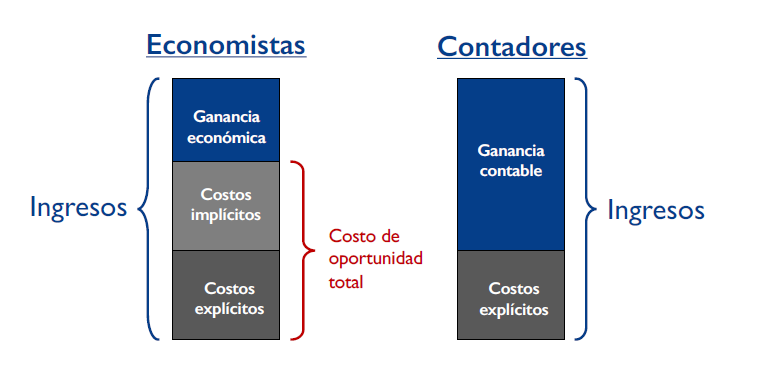
\includegraphics[scale=0.6]{Slides Principios de Economia/Figures/Tema_06.13_beneficioeconomicovscontable.png}
\end{frame}

\begin{frame}
\frametitle{Alta ganancia contable, baja ganancia económica}
\centering
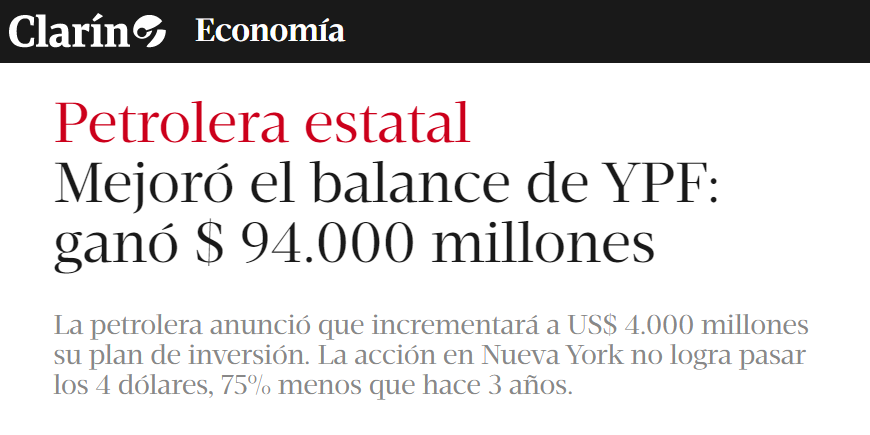
\includegraphics[scale=0.6]{Slides Principios de Economia/YPF.png}
\end{frame}



\begin{frame}
\frametitle{La función de producción en el corto plazo...}
\centering
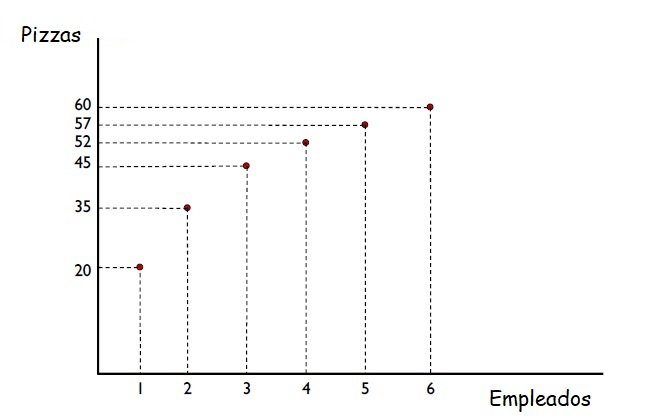
\includegraphics[scale=0.6]{Slides Principios de Economia/Figures/Tema_06.14_funciondeproduccionmedialunas.jpg}
\end{frame}

\begin{frame}
\frametitle{La función de producción de pizzas}
\centering
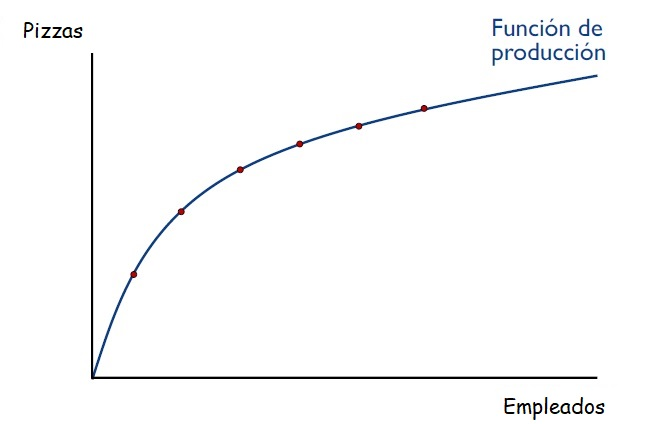
\includegraphics[scale=0.6]{Slides Principios de Economia/Figures/Tema_06.15.jpg}
\end{frame}

\begin{frame}
\frametitle{Contratando a un empleado adicional}
\centering
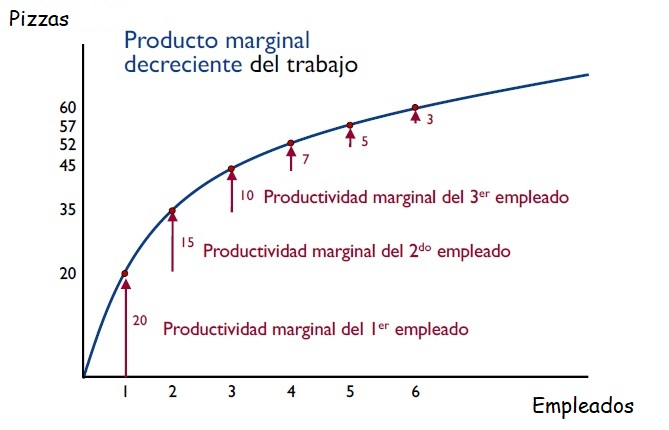
\includegraphics[scale=0.6]{Slides Principios de Economia/Figures/Tema_06.16.jpg}
\end{frame}

\begin{frame}
\frametitle{Producto marginal y medio}
\centering
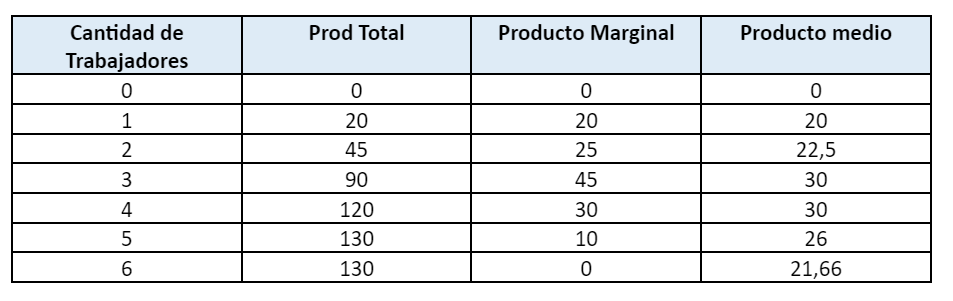
\includegraphics[scale=0.6]{Slides Principios de Economia/Figures/Prod1.png}
\end{frame}


\begin{frame}
\frametitle{Producto medio}
\centering
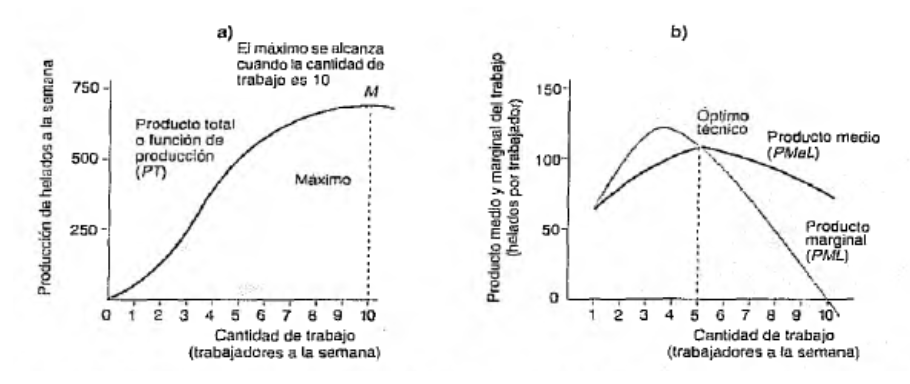
\includegraphics[scale=0.6]{Slides Principios de Economia/Figures/Prod2.png}
\end{frame}

\begin{frame}{Producción y costos}
\begin{itemize}
    \item La función de producción tiene una representación como función de costos
      \item Los costos son de dos tipos
      \begin{itemize} 
      \item Los costos fijos (no cambian con la producción)
      \item Los costos variables (cambian con la producción)
      \end{itemize}
\end{itemize}
\end{frame}

\begin{frame}
\frametitle{Veamos los costos fijos...}
\centering
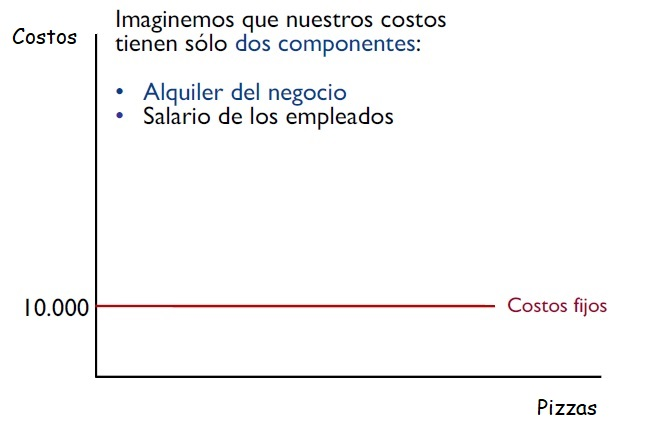
\includegraphics[scale=0.6]{Slides Principios de Economia/Figures/Tema_06.17.jpg}
\end{frame}

\begin{frame}
\frametitle{y ahora los costos variables}
\centering
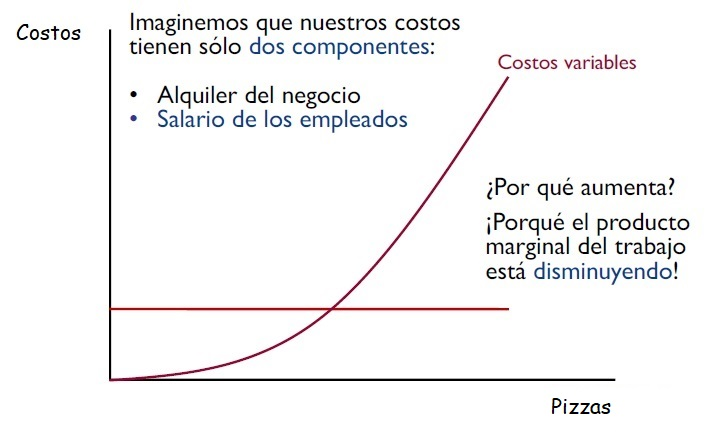
\includegraphics[scale=0.6]{Slides Principios de Economia/Figures/Tema_06.18.jpg}
\end{frame}

\begin{frame}
\frametitle{Los costos totales}
\centering
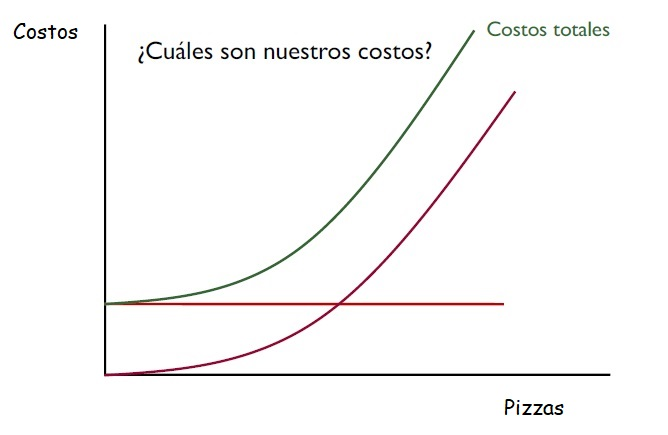
\includegraphics[scale=0.6]{Slides Principios de Economia/Figures/Tema_06.19.jpg}
\end{frame}

\begin{frame}
\frametitle{Los costos de hacer pizzas}
\begin{itemize}
    \item Se observan dos tipos de costos: 
        \begin{itemize}
        \item Los costos fijos
        \item Los costos variables
        \end{itemize}
    \vspace{2mm}
    \item Para evaluar la cantidad de pizzas que queremos producir nos vamos a hacer dos preguntas:
        \begin{itemize}
        \item ¿Cuánto cuesta en promedio una pizza? (Costo medio)
        \item ¿Cuánto cuesta hacer una pizza adicional? (Costo marginal)
        \end{itemize}
\end{itemize}
\end{frame}

\begin{frame}
\frametitle{Costos: ¡para completar! }
\centering
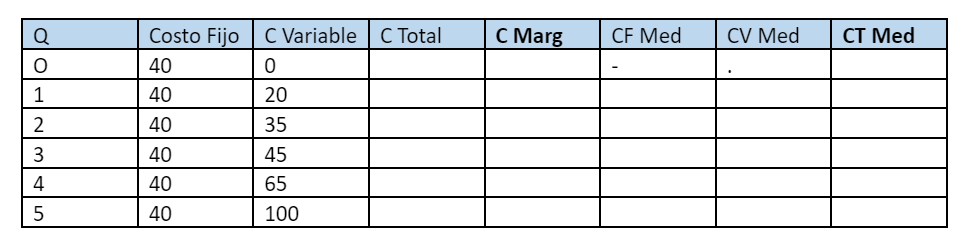
\includegraphics[scale=0.6]{Slides Principios de Economia/Figures/Cost1.png}
\end{frame}

\begin{frame}
\frametitle{Los costos medios y marginales}
\begin{itemize}
    \item El costo medio es el costo promedio por unidad producida
    \begin{itemize}
        \item Gráficamente es la pendiente del rayo que sale desde el origen a un punto dado de la función de costo \\
        - En el ejemplo, disminuye al principio pero luego aumentan 
    \end{itemize}
    \item El costo marginal mide el efecto sobre el costo total al producir una unidad adicional
    \begin{itemize}
        \item Gráficamente, es la pendiente de la función de costo en un punto dado \\
        - En el ejemplo, los costos marginales aumentan a medida que aumenta la producción
    \end{itemize}
\end{itemize}
\end{frame}

\begin{frame}
\frametitle{¿Cómo construir los costos medios?}
\centering
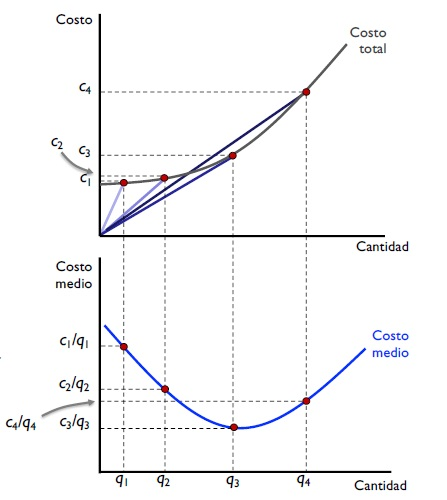
\includegraphics[scale=0.6]{Slides Principios de Economia/Figures/Tema_06.21_funciondeproduccionmedialunas7.jpg}
\end{frame}

%$\begin{frame}
%\frametitle{¿Cómo construir el costo marginal?}
%\centering
%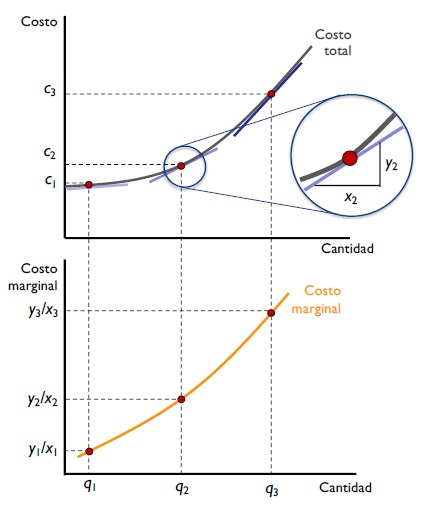
\includegraphics[scale=0.6]{Slides Principios de Economia/Figures/Tema_06.26_costos5.jpg}
%\end{frame}

\begin{frame}
\frametitle{¿Cómo construir el costo marginal?}
\centering
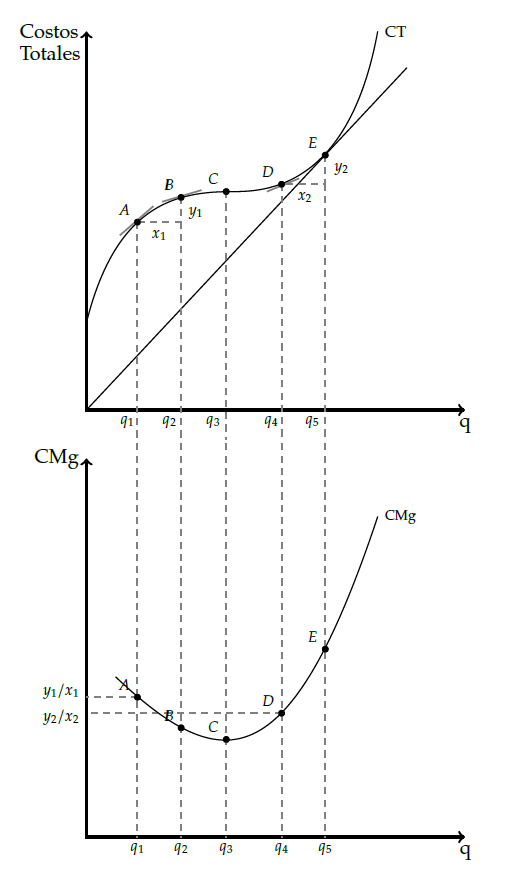
\includegraphics[scale=0.9]{Slides Principios de Economia/Figures/Contruyendocmg.png}
\end{frame}

\begin{frame}
\frametitle{Graficando costo medio y marginal en el mismo gráfico}
\centering
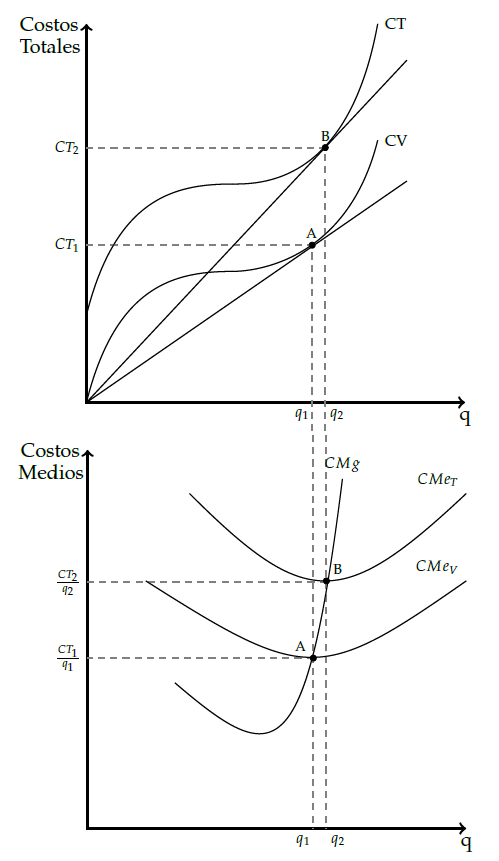
\includegraphics[scale=0.9]{Slides Principios de Economia/Figures/Costoscp.png}
\end{frame}

%\begin{frame}
%\frametitle{Los costos del negocio}
%\centering
%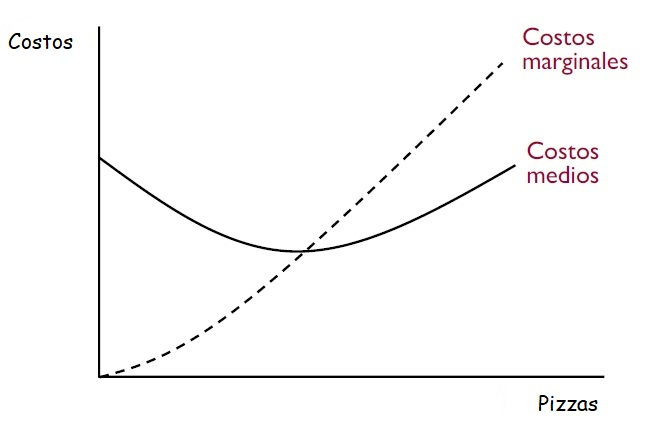
\includegraphics[scale=0.6]{Slides Principios de Economia/Figures/Tema_06.20.jpg}
%\end{frame}

\begin{frame}
\frametitle{Las propiedades de las curvas}
\begin{itemize}
    \item El costo marginal eventualmente aumenta debido a los rendimientos marginales decrecientes.
    \item La curva de costo total promedio suele tener forma de U. Bajan los costos fijos medios y aumentan los costos fijos medios variables.
    \item La curva de costo marginal corta la curva de costo total promedio en su nivel mínimo.
    \item Si el costo marginal es menor al costo medio, el costo medio disminuye al aumentarla producción
\end{itemize}
\end{frame}

\begin{frame}
\frametitle{El error de confundir Cme con Cmg}
\begin{itemize}
    \item Nos enteramos que la universidad cuenta con un centro de llamadas que ya no usa.
    \item Al consultar a las autoridades, responden: «Bueno, una llamada cuesta \$200, mientras que mandar una carta cuesta \$100 ». 
    \item ¿Cómo calculo el costo? Para estimar el costo, la Universidad sumó el costo del sistema informático de telefonía que había comprado años antes y el costo de pagar a estudiantes para realizar las llamadas, y dividieron esa cifra entre el número total de llamadas.
    \item ¿Cuál es el error?
\end{itemize}
\end{frame}


%\begin{frame}
%\frametitle{La curva de oferta del mercado de pizzas}
%\centering
%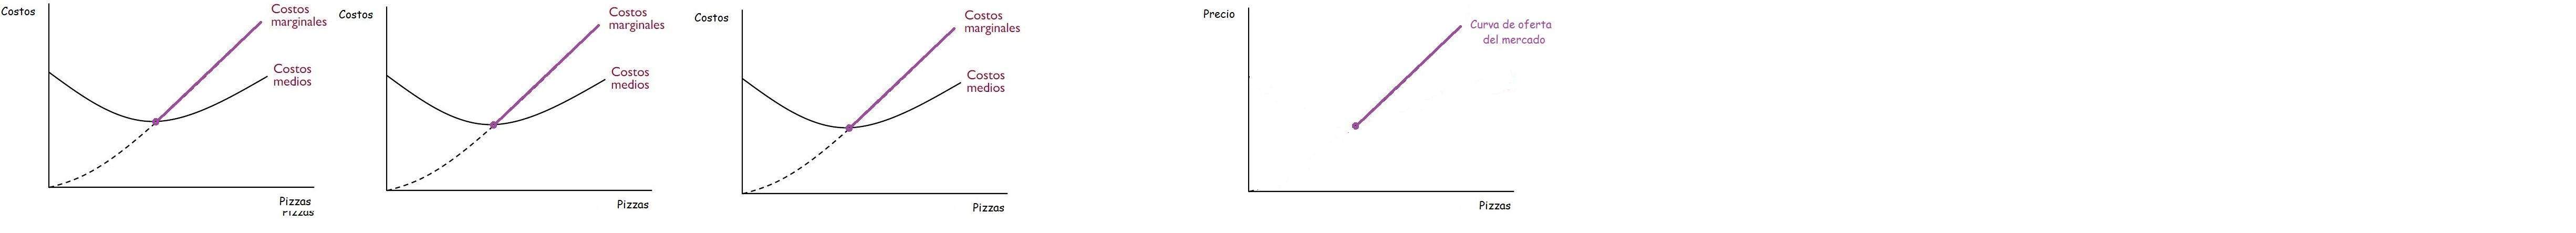
\includegraphics[scale=0.15]{Slides Principios de Economia/Figures/Tema_06.29.jpg}
%\end{frame}


\end{document}


